Variables are just names that point to a memory location. It is used to store data. Its value can be changed, and it can be reused many times. Variable is a way to represent memory location through symbol so that it can be identified easily.

\par Declaration of variables: Announcing the propoerties of variable to the compiler

Properties: 
\begin{itemize}
    \item Size of the variable
    \item Name of the variable
\end{itemize}

Data type: how much space a variable is going to occupy in memory.

\par Definition of variables: Allocating memory to a variable.
Most of the time declaration and definition will be done at the same time.


Initialization of variables: Initializing a variable means specifying an initial value to assign to it (i.e., before it is used at all).\\
Notice that a variable that is not initialized does not have a defined value, hence it cannot be used until it is assigned such a value. If the variable has been declared but not initialized, we can use an assignment statement to assign it a value.


Variable name: composed of alphabets or combination of letters and digits.

Variable naming conventions: 
\begin{enumerate}
    \item Don't start variable name with digit.
    \item Beginning with underscore is valid but not recommended.
    \item C language is case sensitive.
    \item Special characters except underscore are not allowed in the variable name.
    \item Blanks or white spaces not allowed.
    \item Don't use keywords to name your variables.
    \item Don't use long names your variables.
    \item Redefinition of a variable is not allowed.
\end{enumerate}


Scope of variables: 

Scope of variables refers to the area of the program where the variables can be accessed post declaration. In other words, a block or a region where a variable is declared, defined and used and when a region ends, variable is automatically destroyed.

In C, every variable defined in scope. You can define scope as the section or region of a program where a variable has its existence; moreover, that variable cannot be used or accessed beyond that region.

Scope of a variable:   
Local scope or Block scope
A local scope or block scope is collective program statements put in and declared within a function or block (a specific region enclosed with curly braces) and variables lying inside such blocks are termed as local variables. 

Variable(s) that are declared within a block can be accessed within that specific block and all other inner blocks of that block, but those variables cannot be accessed outside the block.

\begin{figure}[H]
    \begin{center}
        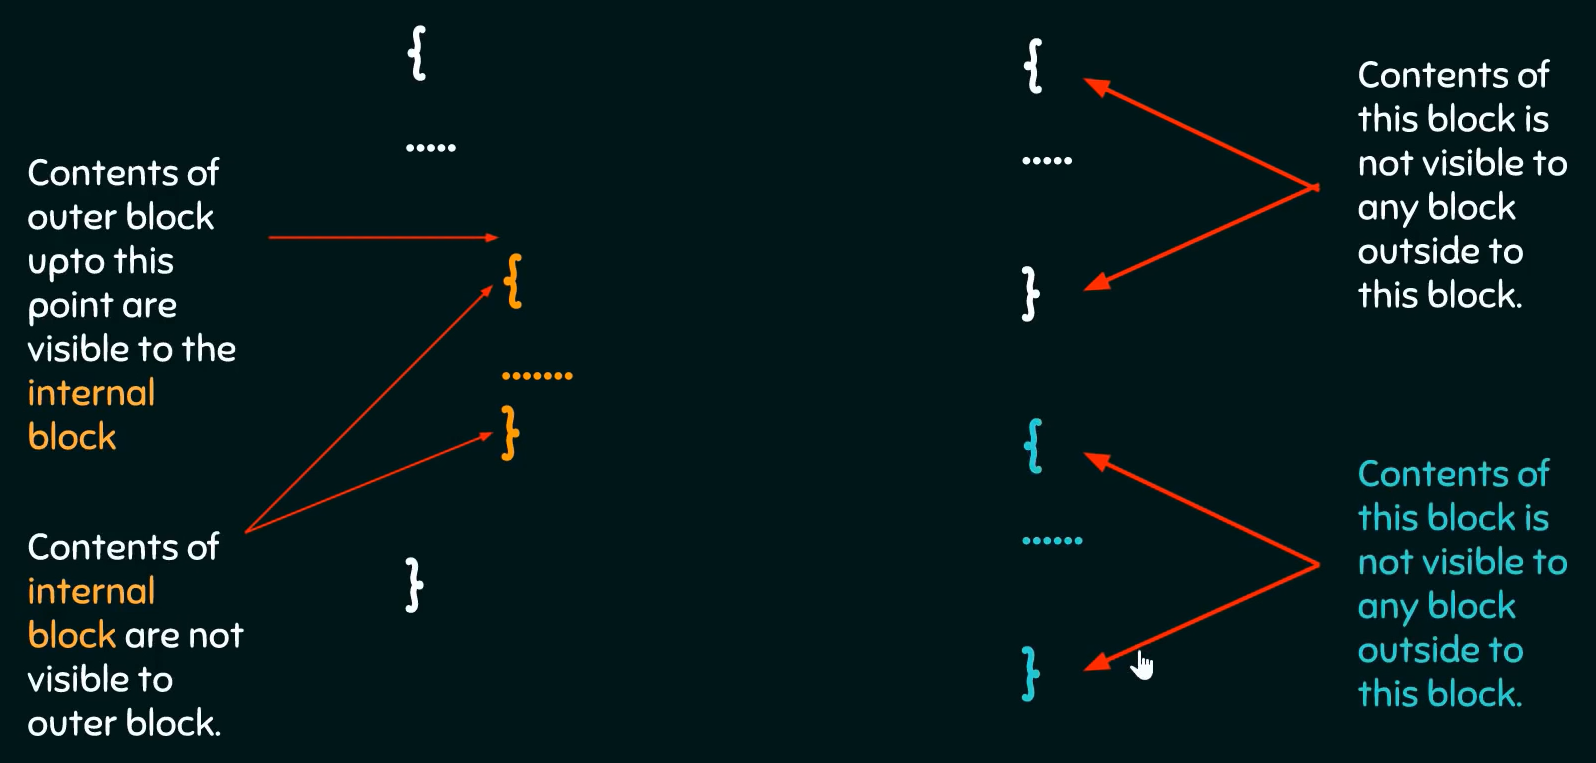
\includegraphics[width=\textwidth]{images/variableScope.png}
        \caption{Scope of a variable}
        \label{variableScope}
    \end{center}
\end{figure}

Local Variable
Variables that are declared within the function block and can be used only within the function are called local variables.

Global variable
Variables that are declared outside of all function blocks and can be accessed inside all the functions are called global variables.

\subsection{Data types}
\begin{itemize}
    \item Exceeding the valid range of data type:
    Let us say that the max number of bytes in a particular data type is 'n'. Exceeding the range of the data type means that assigning a number with bits greater than 'n' bits. Hence, (MSB) bits beyond 'n' bits will be missed.

    \item \textbf{Range} is nothing but upper and lower limits of some set of data. Binary: \(2^{n} - 1\), where, n is number of buts.
    Unsigned range: o to 65535 2 bytes
    Signed range: -32768 to +32767\\ 

    \item \textbf{sizeof()} is a unary operator (not a function) that  can get the size of a data type programmatically.\\
    \textbf{Modifiers for integers (short, long, signed, unsigned)}\\
    \textbf{long \& short} are modifiers which are used to take either less or more memory.

    \item Number systems 
    \begin{itemize}
        \item Decimal number system: Human understandable number system. Also, called as base 10  number system. Range 0 to 9.
        \item Binary number system: Computer understandable number system. Also, called as base 2 number system. Range 0 to 1.
    \end{itemize}       

    \item \textbf{Fixed point and Floating point representation}
    Fixed point and floating point are two ways of representing fractional numbers. 
    \begin{itemize}
        \item In fixed point, there is a specific number of digits to represent the integer section and fraction section  i.e. the decimal point has a fixed location. 
        \item In floating point, there is no specific number of digits to represent integer section and fraction section i.e. the decimal point is floating. A number in floating point representation is as follows:
        \(+/- Mantissa * 10^{exponent}\)
    \end{itemize}
\end{itemize}

\begin{figure}[H]
    \begin{center}
        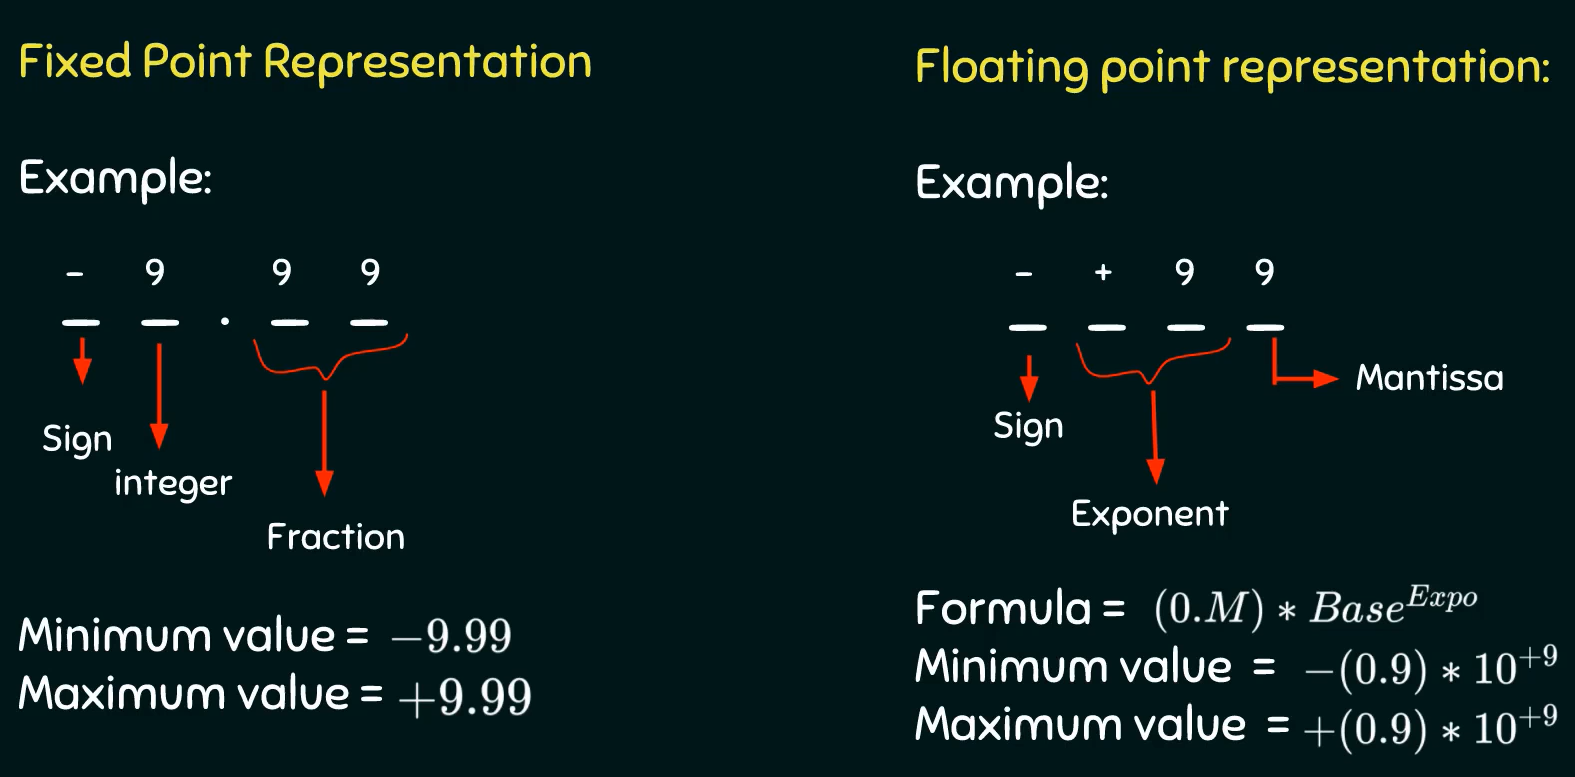
\includegraphics[width=\textwidth]{images/fixedFloating.png}
        \caption{Fixed point and Floating point representation}
        \label{fixedFloating}
    \end{center}
\end{figure}


\subsubsection{integer}

\begin{itemize}
    \item integer data type is used to represent integers.
    \item Syntax: int variable\_name; (by default variable is chosen as a signed integer)\\
    Unsigned int declaration: unsigned int variable\_name; \\
    \item Format specifier: 
    \begin{itemize}
        \item int = "\%d" (signed int)
        \item short int = "\%d" (signed short int)
        \item long int = "\%ld" (signed long int)
        \item unsigned int = "\%u" (unsigned int)
        \item short unsigned int = "\%u" (unsigned short int)
        \item long unsigned int = "\%lu" (unsigned long int)
    \end{itemize} 
    \item size: Integer can take either 2 or 4 bytes of memory. (vary as per system)
    \begin{itemize}
        \item int = 4
        \item short int = 2
        \item long int = 8
    \end{itemize} 
    \item Range: Unsigned: 0 to 255 \& Signed: -128 to +127
    \item sizeof(short int) <= sizeof(int) <= sizeof(long int)
\end{itemize}


\subsubsection{Character}
\begin{itemize}
    \item Character data type is used to represent characters.
    \item Representation: Characters are encoded using ASCII encoding scheme into 8 bit binary representation. There are 2 types of ASCII encoding schemes:
    \begin{itemize}
        \item Traditional ASCII: 7 bit representation MSB is always zero
        \item Extended ASCII: 8 bit representation of characters
    \end{itemize}
    \item Syntax: char variable\_name = 'N';
    \item Character data type can hold a single character and cannot hold a string.
    \item Format specifier: "\%c"
    \item size: 1 byte
    \item Range: Unsigned: 0 to 255 \& Signed: -128 to +127
\end{itemize}

Signed characters: 2's complement representation
Unsigned characters:

\subsubsection{float}
\begin{itemize}
    \item float data type is used to represent fractional numbers.
    \item Representation: IEEE 754 Single Precision Floating Point
    \item Syntax: float variable\_name = 'fractional number';
    \item float data type has a precision of upto 8 decimals(including decimal point and integer)
    \item Format specifier: "\%f"
    \item size: 4 bytes (vary as per system)
\end{itemize}


\subsubsection{double}
\begin{itemize}
    \item double data type is used to represent fractional numbers.
    \item Representation: IEEE 754 Double Precision Floating Point
    \item Syntax: double variable\_name = 'fractional number';
    \item double data type has a precision of upto 16 decimals(including decimal point and integer)
    \item Format specifier: "\%f" or  "\%lf"
    \item size: 8 bytes (vary as per system)
\end{itemize}

\subsubsection{long double}
\begin{itemize}
    \item long double data type is used to represent fractional numbers.
    \item Representation: Extended Precision Floating Point
    \item Syntax: long double variable\_name = 'fractional number';
    \item long double data type has a precision of upto 32 decimals(including decimal point and integer)
    \item Format specifier: "\%Lf"
    \item size: 16 bytes (vary as per system)
\end{itemize}


\section{Variable Modifiers}

\subsection{Auto}
\begin{itemize}
    \item Auto stands for Automatic.
    \item Syntax: auto int variable\_name;
    \item Variables declared inside a scope by default are automatic variables. Automatic variable is a variable which automatically gets destroyed after the completion of a function or a scope in which it is defined.
    \item Advantage: This variable does not waste memory.
    \item If auto variable is not initialized, it will be assigned a random value by default. Whereas, a global variable is initialized to 0 by default.
\end{itemize}

\subsection{Extern modifier}
\begin{itemize}
    \item Extern is a short for External.
    \item Syntax: (declaration) extern int variable\_name; (no memory is allocated.)
    \item Extern is used when a particular file needs to access a variable from another file.
    \item When an extern variable is initialized, then memory for this variable is allocated and it will be considered defined.
\end{itemize}

\subsection{Register}
\begin{itemize}
    \item Register keyword hints the compiler to store a variable in register memory.
    \item Syntax: register data\_type variable\_name;
    \item Access time reduces greatly for most frequently referred variables.
    \item To put or to not put a variable in register is the choice of compiler.
    \item Usually compiler do the necessary optimizations.
\end{itemize}

\subsection{Static}
\begin{itemize}
    \item Static variables have a property of preserving their value even after they are out of their scope. Hence, static variables preserve their previous value in their previous scope and are not initialized again in the new scope. 
    \item Syntax: static   = variable\_value; 
    \item  A static int variable remains in memory while the program is running. A normal or auto variable is destroyed when a function call where the variable was declared is over. 
    \item Static variables (like global variables) are initialized as 0 if not initialized explicitly.
    \item Static variables are allocated memory in data segment, not stack segment.
    \item Static global variables and functions are also possible in C/C++. The purpose of these is to limit scope of a variable or function to a file.
    \item Static variables should not be declared inside structure. 
\end{itemize}